\documentclass[class=report, crop=false, 12pt,a4paper]{standalone}
\usepackage{enumitem}
\usepackage{float}
\usepackage[normalem]{ulem}
\usepackage{graphicx}
\usepackage{amsmath}
\usepackage{siunitx}
\usepackage{commath}
\usepackage{tikz}
\usetikzlibrary{positioning, fit, calc}   
\tikzset{block/.style={draw, thick, text width=3cm ,minimum height=1.3cm, align=center},   
line/.style={-latex}     
}  
\begin{document}
\section{Centrifugal pumps}
\subsection{Functional principle}
Centrifugal pump's working principle can be understood very simply if you think about what happens to the liquid level when you steer a liquid in a glass: the free surface of the liquid becomes concave, and rises from the centre to the periphery - you are raising the flow head at the periphery.
\subsection{Functional components}
\begin{figure}[H]
  \centering
  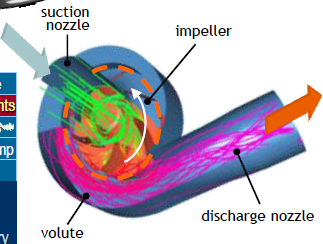
\includegraphics[width = 0.6\textwidth]{../img/diagram1.png}
\end{figure}
The fluid enters axially and receives tangential and radial velocity by momentum transfer from rotating blades. The centrifugal force provides further radial velocity. Then the flow is collected and decelerated, in order to increase its pressure before it leaves the pump. The process produces depression at the pump axis, which sucks new fluid. The functional components of centrifugal pumps are:
\begin{itemize}
  \item \textbf{The suction nozzle}: leads the fluid from pump inlet to the impeller eye. It is usually a cylindrical or truncated conical tube and can have stationary vanes to induce some spinning to the suction flow
  \item \textbf{The impeller}: it is rotating component that provides momentum to the fluid. It can have many different features, that we will analyse in more detail later on
  \item \textbf{The volute (or scroll)}: decelerates the fluid, converting the momentum into pressure, and delivers it to the discharge pipe. It has a gradually enlarging section (which gives its snail-shape) and can have stationary blades
\end{itemize}
\subsection{Pumps arrangement}
We have already mentioned the main functional limitations of roto-dynamic pumps over positive-displacement pumps:
\begin{itemize}
  \item Adjustment o capacity requires changes in the operating speed and affects the efficiency
  \item The net head is lower and its adjustment requires significant changes in the operating speed and efficiency
\end{itemize}
These limitations can be overcome by using two or more pumps in \textbf{parallel} or in \textbf{series}.
\begin{itemize}
  \item \textbf{Pumps operating in parallel}: two or more pumps are used to draw fluid from the same source and discharge it to a single pipe. This arrangement allows variable discharge arrangement in terms of capacity
  \item \textbf{Pumps operating in series}: the discharge from one pump is piped into the suction nozzle of a flowing pump. Each pump adds energy to the same fluid, increasing the final net head. Efficiency decrease for more than 10-12 impellers
\end{itemize}
\begin{figure}[H]
  \centering
  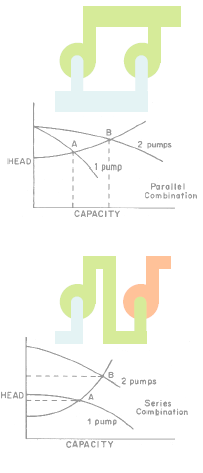
\includegraphics[width = 0.3\textwidth]{../img/diagram2.png}
\end{figure}
\subsection{End-suction pump}
\begin{figure}[H]
  \centering
  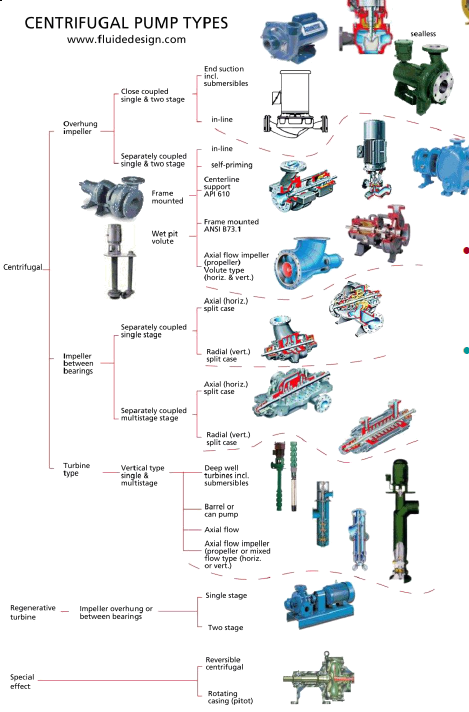
\includegraphics[width = 0.5\textwidth]{../img/diagram3.png}
\end{figure}
The different operating requirements have produced a large number of possible centrifugal pump designs. We will consider the most common version, which is called \textbf{end-suction centrifugal pump}, and consists of the following parts:
\begin{itemize}
  \item A rotating component called rotor (red)
  \begin{itemize}
    \item Impeller blades, hub and shroud
    \item Shaft
  \end{itemize}
  \item A stationary component (green)
  \begin{itemize}
    \item Suction nozzle
    \item Scroll casing (or volute casing)
    \item Pump casing
    \item Back cover
    \item Bearings
  \end{itemize}
\end{itemize}
\begin{figure}[H]
  \centering
  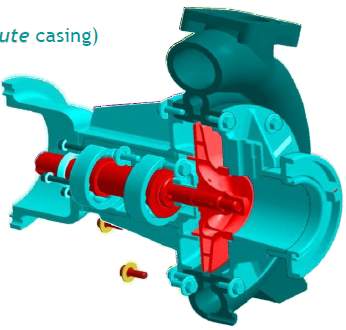
\includegraphics[width = 0.7\textwidth]{../img/diagram4.png}
  \caption{End-suction centrifugal pump}
\end{figure}
\subsection{The Impeller}
The \textbf{impeller} is the rotating component that provides the momentum to the fluid. It can be classified based on the major direction of the flow at the exit from the blades.
\begin{itemize}
  \item Axial flow - the flow leaves the impeller parallel to the axis of rotation
  \item Mixed flow - the flow leaves the impeller at an angle with the axis of rotation
  \item Radial flow - the flow leaves the impeller orthogonal to the axis of rotation
\end{itemize}
It can be classified based on the suction type.
\begin{itemize}
  \item Single suction - the liquid inlet to the impeller is on one side only
  \item Double suction - the liquid inlet to the impeller is symmetrical from two sides. The provides a very stable hydraulic performance because the hydraulic forces are balanced
\end{itemize}
It can be classified based on the presence of shrouds.
\begin{itemize}
  \item Open impeller - blades are supported almost entirely by the impeller hub. It is primarily applied to clean, non-abrasive, low-horsepower applications and operates at a high efficiency
  \item Enclosed impeller - incorporates a full front and back shroud. Fluid flows without hydraulic interaction with the casing walls. The friction caused by the small gap between shroud and casing reduces efficiency
  \item Semi-closed impeller - incorporates a single shroud, usually located on the back of the impeller. It is more efficient than an enclosed impeller (lower disc friction and tighter axial clearances). Compared to an open impeller it can be adjusted axially to compensate for casing wear. We will be designing one of these
\end{itemize}
It can be classified based on the blade geometry.
\begin{itemize}
  \item Backward inclined - have the highest efficiency (the fluid experiences the minimum amount of turning) and intermediate pressure rise
  \item Radial - produce the highest pressure rise. Pressure rise drops suddenly after the BEP. Efficiency is intermediate
  \item Forward inclined - produce a lower but more constant pressure rise over different flow rates. Efficiency is lower
\end{itemize}
\subsection{Flow into the impeller}
The design of the blades has  to take into account the velocity flow through the impeller: The flow field into the impeller is:
\begin{itemize}
  \item Unsteady
  \item Fully three-dimensional
  \item May be compressible
\end{itemize}
Assumptions:
\begin{itemize}
  \item Steady flow
  \item We do not consider axial velocity - we consider only the normal ($n$) and tangential ($t$) components in the impeller plane
  \item We consider incompressible flow
  \item No leakage - in practice leakage will be considered by increasing the volume flow rate using in the design calculation
  \item We consider the flow to be always tangential to the blades surface when viewed from a reference frame rotating with the blades (shockless entry and no flow separation)
\end{itemize}
Efficient designs are aimed at accommodating the fluid flow into the impeller. The flow velocities into the impeller ensure the requirements to be met (are linked to $Q$ and $H$) and are the combination of:
\begin{itemize}
  \item Velocity of the fluid 'relative' to the blades
  \item Velocity of the blades
\end{itemize}
\textbf{Velocities of the blades} are known both in direction and magnitude, everywhere in the impeller.
\begin{itemize}
  \item Direction: orthogonal to the radius (tangential direction)
  \item Magnitude: depending on the angular velocity $\omega$ of the impeller and on the local radius $r$.
\end{itemize}
\begin{gather}
  v_{r \textrm{, blade}} = \omega r\\
  V_{1 \textrm{, blade}} = \omega r_1\\
  V_{2 \textrm{, blade}} = \omega r_2\\
\end{gather}
\begin{figure}[H]
  \centering
  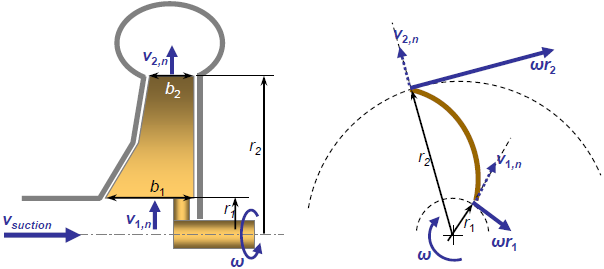
\includegraphics[width = 0.7\textwidth]{../img/diagram5.png}
\end{figure}
\textbf{Velocities of the flow relative to the blades}, we know the radial component and the direction. Due to conservation of mass and incompressibility assumption. The flow rate at each radius has to be the same (equal to the suction flow rate).
\begin{gather}
  \textrm{if } Q = A_{\textrm{suction}} \times v_{\textrm{suction}}\\
  Q = 2 \pi r_1 b_1 \times v_{1, n} = 2\pi r_2 b_2 \times v_{2, n}\\
  v_{2, n} = v_{1, n} \frac{r_1 b_1}{r_2 b_2}
\end{gather}
where subscript $n$ signifies the normal component.
\begin{figure}[H]
  \centering
  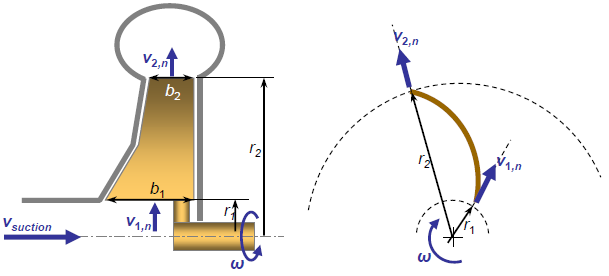
\includegraphics[width = 0.7\textwidth]{../img/diagram6.png}
\end{figure}
\begin{itemize}
  \item Direction: due to no-separation condition, direction is parallel to the blade surfaces
  \item At the inlet and outlet edges ($v_{1, rel}$ and $v_{2, rel}$) they form angles with the tangential direction respectively equal to $\beta_1$ and $\beta_2$
\end{itemize}
\begin{figure}[H]
  \centering
  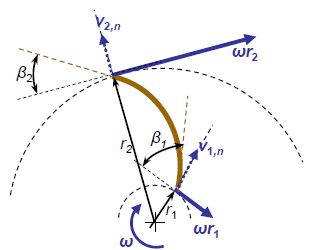
\includegraphics[width = 0.5\textwidth]{../img/diagram7.png}
\end{figure}
The leading edge angle $\beta_1$ is defined as the blade angle relative to the reverse tangential direction at radius $r_1$ and the trailing edge angle $\beta_2$ as the blade angle relative to the reverse tangential direction at radius $r_2$. We can combine all information and apply the parallelogram rule to calculate
\begin{itemize}
  \item The magnitude of $v_{1, rel}$ and $v_{2, rel}$
  \item The absolute fluid velocities $V_1$ and $V_2$ in direction and magnitude
\end{itemize}
\begin{figure}[H]
  \centering
  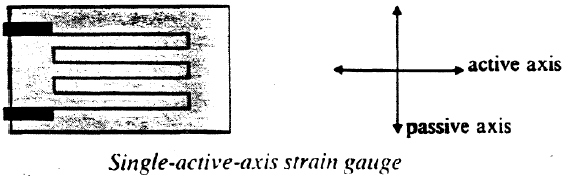
\includegraphics[width = 0.8\textwidth]{../img/diagram10.png}
\end{figure}
The normal and tangential components of the absolute velocity are:
\begin{gather}
  v_{2,n} = v_{2,rel} \sin{\beta} \\
  v_{2,t} = (v_{2,\textrm{blade}} - v_{2, rel} \cos{\beta}) = \omega r_2 - v_{2,rel}\cos{\beta}
\end{gather}
The normal components of the inlet and outlet velocities are directly related to the capacity through the conservation equation. The tangential components of the inlet and outlet velocities are directly related to the torque and to the required head through the Euler's turbomachine equation. A similar equation is found at the blade inlet.
\subsection{Euler's turbomachine equation}
To calculate the torque $T_{\textrm{shaft}}$ on the rotating shaft, the angular momentum relation is used. The starting point to obtain it is Newton's second law: the amount of force exerted upon the object is directly proportional to the rate of change in the momentum of the object.
\begin{equation}
  \vec{F} = \frac{d}{dt}(m\vec{v})
\end{equation}
The moment of a force $\vec{F}$ about a point $O$ is given by $\vec{T} = \vec{r}\times\vec{F}$, where $\vec{r}$ is the vector from $O$ to $\vec{F}$ called radius vector (where $\times$ is cross product). From the two expressions:
\begin{equation}
  \vec{T} = \vec{r} \times \frac{d}{dt} (mv)
\end{equation}
We define a vector $\vec{L}$ called angular momentum as vector product of the radius vector to the object and the linear momentum of the object.
\begin{equation}
  \vec{L} = \vec{r} \times m \vec{v}
\end{equation}
Upon taking the temporal differential of $\vec{L}$, we have: 
\begin{equation}
  \frac{d\vec{L}}{dt} = \frac{d\vec{r}}{dt} \times m\vec{v} + \vec{r} \times \frac{d}{dt}(m\vec{v})
\end{equation}
But $ \frac{d\vec{r}}{dt} = \vec{v}$ and the cross product of parallel vectors is 0. Therefore:
\begin{equation}
  \vec{T} = \frac{d\vec{L}}{dt}
\end{equation}
The rate of change of angular momentum of an object about a fixed point is equal to the torque applied to the object.
\subsection{Flow into the impeller}
\begin{figure}[H]
  \centering
  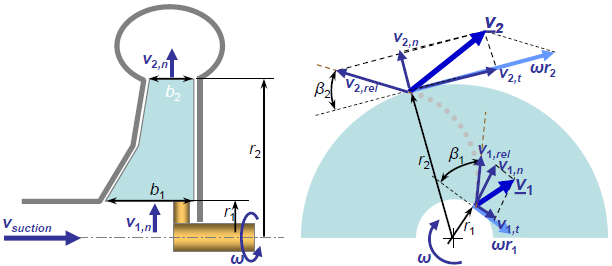
\includegraphics[width = 0.8\textwidth]{../img/diagram9.png}
  \caption{Consider the control volume described by the rotating impeller blades.}
\end{figure}
We can calculate the torque $T_{\textrm{shaft}}$ on the rotating shaft from the Euler turbomachine equation:
\begin{equation}
  T_{\textrm{shaft}} = \rho Q (r_2 v_{2,t} - r_1 v_{1,t})
\end{equation}
Assuming no losses, the efficiency is equal to one and therefore the ideal net head of the pump can be calculated as:
\begin{gather}
  \eta_{\textrm{pump}} = \frac{\rho g Q}{\omega T_{\textrm{shaft}}}H = 1\\ 
  \rho g QH = \omega T_{\textrm{shaft}} = \omega\rho Q (r_2v_{2,t} - r_1 v_{1,t})\\
  H = \frac{1}{g}(\omega r_2 v_{2,t} - \omega r_1 v_{1,t})
\end{gather}
The operating conditions of the pump are related to the flow velocities into the impeller:
\begin{gather}
  \textrm{Flow rate: } Q = 2\pi r_1 b_1 b_{1,n} = 2\pi r_2 b_2 v_{2,n}\\
  \textrm{Ideal head: } H = \frac{1}{g}(\omega r_2 v_{2,t} - \omega r_1 v_{1,t})
\end{gather}
Since the flow velocities into the impeller depend on the blades angles (e.g. leading and trailing edge angles) the impeller cna be designed in order to match required operative conditions.
\begin{gather}
  v_{1,2,n} = v_{1,2,rel} \sin{\beta_{1,2}}\\
  v_{1,2,n} = (v_{1,2,\textrm{blade}} - v_{1,2,rel} \cos{\beta_{1,2}}) = \omega r_{1,2} - v_{1,2,rel} \cos{\beta_{1,2}}
\end{gather}
$Q, \ H, \ v_n, \ v_t$ are in terms of $r, \ b, \ \omega, \ \beta, \ v_{rel}$
\end{document}